\subsection{Die Zeitkonstante des RC-Gliedes}
Im ersten Veruchsteil soll die Zeitkonstante $\tau$ eines RC-Gliedes bestimmt werden.
Hierzu wird der Entladevorgang des Kondensators bei angelegter Rechteckspannung untersucht.
Die entsprechende Schaltung mitsamt Oszilloskop ist in Abbildung \ref{fig:zeitkonst} zu sehen.
\begin{figure}[H]
    \centering
    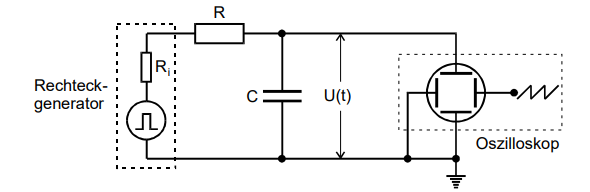
\includegraphics[height=5cm]{abbildungen/zeitkonstante.png}
    \caption[short]{Schaltung zur Bestimmung der Zeitkonstanten.}
    \label{fig:zeitkonst}
\end{figure}
Der Entladeprozess beginnt, sobald die Rechteckspannung auf Null zurück gesprungen ist, und dauert so lange, wie sie auf Null verharrt\footnote{Ganz 
analog kann auch zur Bestimmung von $\tau$ der Aufladevorgang untersucht werden.
Dieser beginnt beim Sprung der Generatorspannung von Null auf den Maximalwert und dauert so lange, 
wie sie auf diesem Wert verbleibt.}.
Somit werden stets Ausschnitte des eigentlich unendlich langen Vorgangs beobachtet.
Für eine höhere Ablesegenauigkeit werden Rechteckfrequenz und Ablenkgeschwindigkeit des Kathodenstrahls so eingestellt, 
dass ein ganzer Abschnitt möglichst groß auf dem Oszilloskop zu erkennen ist.
%...